\documentclass[fleqn]{article}
\usepackage[margin=1in]{geometry}
\usepackage[nodisplayskipstretch]{setspace}
\usepackage{amsmath, nccmath, bm}
\usepackage{amssymb}
\usepackage{enumitem}
\usepackage{graphicx}
\usepackage{float}
\usepackage{listings}
\usepackage{hyperref}
\usepackage[svgnames]{xcolor}
\graphicspath{{./images}}

\hypersetup{
    colorlinks=true,
    linkcolor=black,
    filecolor=black,      
    urlcolor=blue
    }

\newcommand{\zerodisplayskip}{
	\setlength{\abovedisplayskip}{0pt}%
	\setlength{\belowdisplayskip}{0pt}%
	\setlength{\abovedisplayshortskip}{0pt}%
	\setlength{\belowdisplayshortskip}{0pt}%
	\setlength{\mathindent}{0pt}}
	
\definecolor{vgreen}{RGB}{104,180,104}
\definecolor{vblue}{RGB}{49,49,255}
\definecolor{vorange}{RGB}{255,143,102}

\lstdefinestyle{verilog-style}
{
    language=Verilog,
    basicstyle=\small\ttfamily,
    keywordstyle=\color{vblue},
    identifierstyle=\color{black},
    commentstyle=\color{vgreen},
    numbers=left,
    numberstyle=\tiny\color{black},
    numbersep=10pt,
    tabsize=8,
    moredelim=*[s][\colorIndex]{[}{]},
    literate=*{:}{:}1
}

\lstset{style={verilog-style},showstringspaces=false}

\makeatletter
\newcommand*\@lbracket{[}
\newcommand*\@rbracket{]}
\newcommand*\@colon{:}
\newcommand*\colorIndex{%
    \edef\@temp{\the\lst@token}%
    \ifx\@temp\@lbracket \color{black}%
    \else\ifx\@temp\@rbracket \color{black}%
    \else\ifx\@temp\@colon \color{black}%
    \else \color{vorange}%
    \fi\fi\fi
}
\makeatother

\newcommand{\code}[1]{%
	\colorbox{Gainsboro}{\texttt{#1}}%
}

\title{Homework 4}
\author{Owen Sowatzke}
\date{April 16, 2025}

\begin{document}

	\offinterlineskip
	\setlength{\lineskip}{12pt}
	\zerodisplayskip
	\maketitle
	
	\begin{enumerate}
		\item ~
		
			\begin{figure}[H]
				\centerline{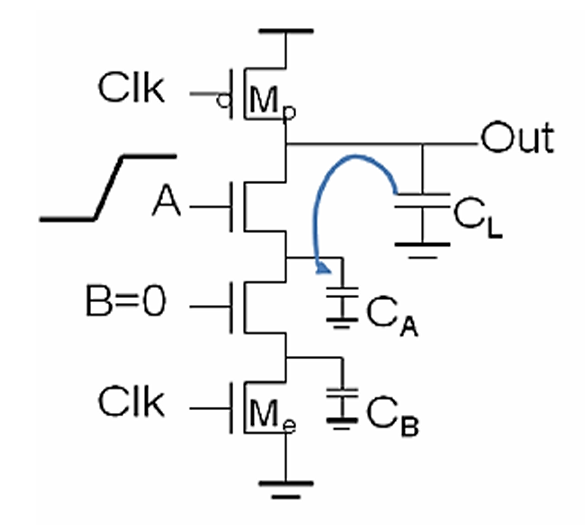
\includegraphics[width=0.5\textwidth]{circuit_question1.png}}
				\label{fig::circuit_question1}
			\end{figure}

			\begin{enumerate}
			\item[1.] Write out the output function in terms of A and B.			
			
			\begin{equation*}
				\mathbf{Out = \overline{AB}}
			\end{equation*}
			
			\item[2.] $V_{DD}=2.0\text{V}$, $|V_{th}|=0.6\text{V}$ for all PMOS and NMOS transistors. $C_L/C_A=3$, $C_L/C_B=5$; What is the voltage value at X and at output nodes ($V_x$ = ? and $V_{out}$ = ?)
			
			$V_{\text{out}}$ will be charged to $V_{DD}$ during the precharge phase. Assume that all other nodes are charged to $0\text{V}$. When $A$ rises from 0 to 1, $C_L$ will discharge through $M_a$ and share charge with $C_A$. Because $B=0$, $M_b$ will be in cutoff mode, and there will be no charge sharing with $C_B$.
			
			Start by assuming that $M_a$ is fully conductive (i.e. there is no voltage drop across it).
			
			\begin{equation*}
				C_LV_{DD} = (C_L + C_A)V_{out} 
			\end{equation*}			
			
			\begin{equation*}
				\Rightarrow V_x = V_{out} = \frac{C_LV_{DD}}{C_L + C_A} = \frac{3C_AV_{DD}}{3C_A + C_A} = \frac{3V_{DD}}{4} = 1.5\text{V}
			\end{equation*}
			
			 However, for $M_a$ to be on $V_{gs} > V_{th} \Rightarrow V_x \leq 1.4\text{V}$.
			
			Therefore, $C_A$ will charge until $V_x$ is 1.4V, all remaining charge will remain in $C_L$.
			
			$\Rightarrow Q_{out} = C_LV_{DD} - C_AV_x = 2C_L - 1.4C_A = 6C_A - 1.4C_A = 4.6C_A$
			
			$\therefore V_\text{out} = Q_{out}/C_L = 4.6C_A/3C_A = \mathbf{1.53\text{\textbf{V}}},\ V_x = \mathbf{1.4\text{\textbf{V}}}$
			
			\end{enumerate}
		
		\item Use static complementary CMOS design, Pseudo-NMOS, domino dynamic design to implement
		
		$\mathbf{Y = \overline{(A + B)C + D}}$
		
		Assume we use short channel transistors. We use 0.10um process with 1GHz clock frequency and 1.0V power supply with 121mA/mm. We would like to keep the power density the same, but we would like to scale current density to $81\text{mA}/\text{mm}^2$.
		
		Our static complementary CMOS design is shown in Figure \ref{fig::problem2_static_cmos}. To design it, we start with the pull-down network. Each OR in our logical equation becomes a parallel set of NMOS transistors, and each AND becomes a series of NMOS transistors. Then to get the pull-up network, we use the rule of conduction complements. Each series of NMOS transistors becomes a parallel set of PMOS transistors, and each parallel set of NMOS transistors becomes a series of PMOS transistors.
		 
		\begin{figure}[H]
			\centerline{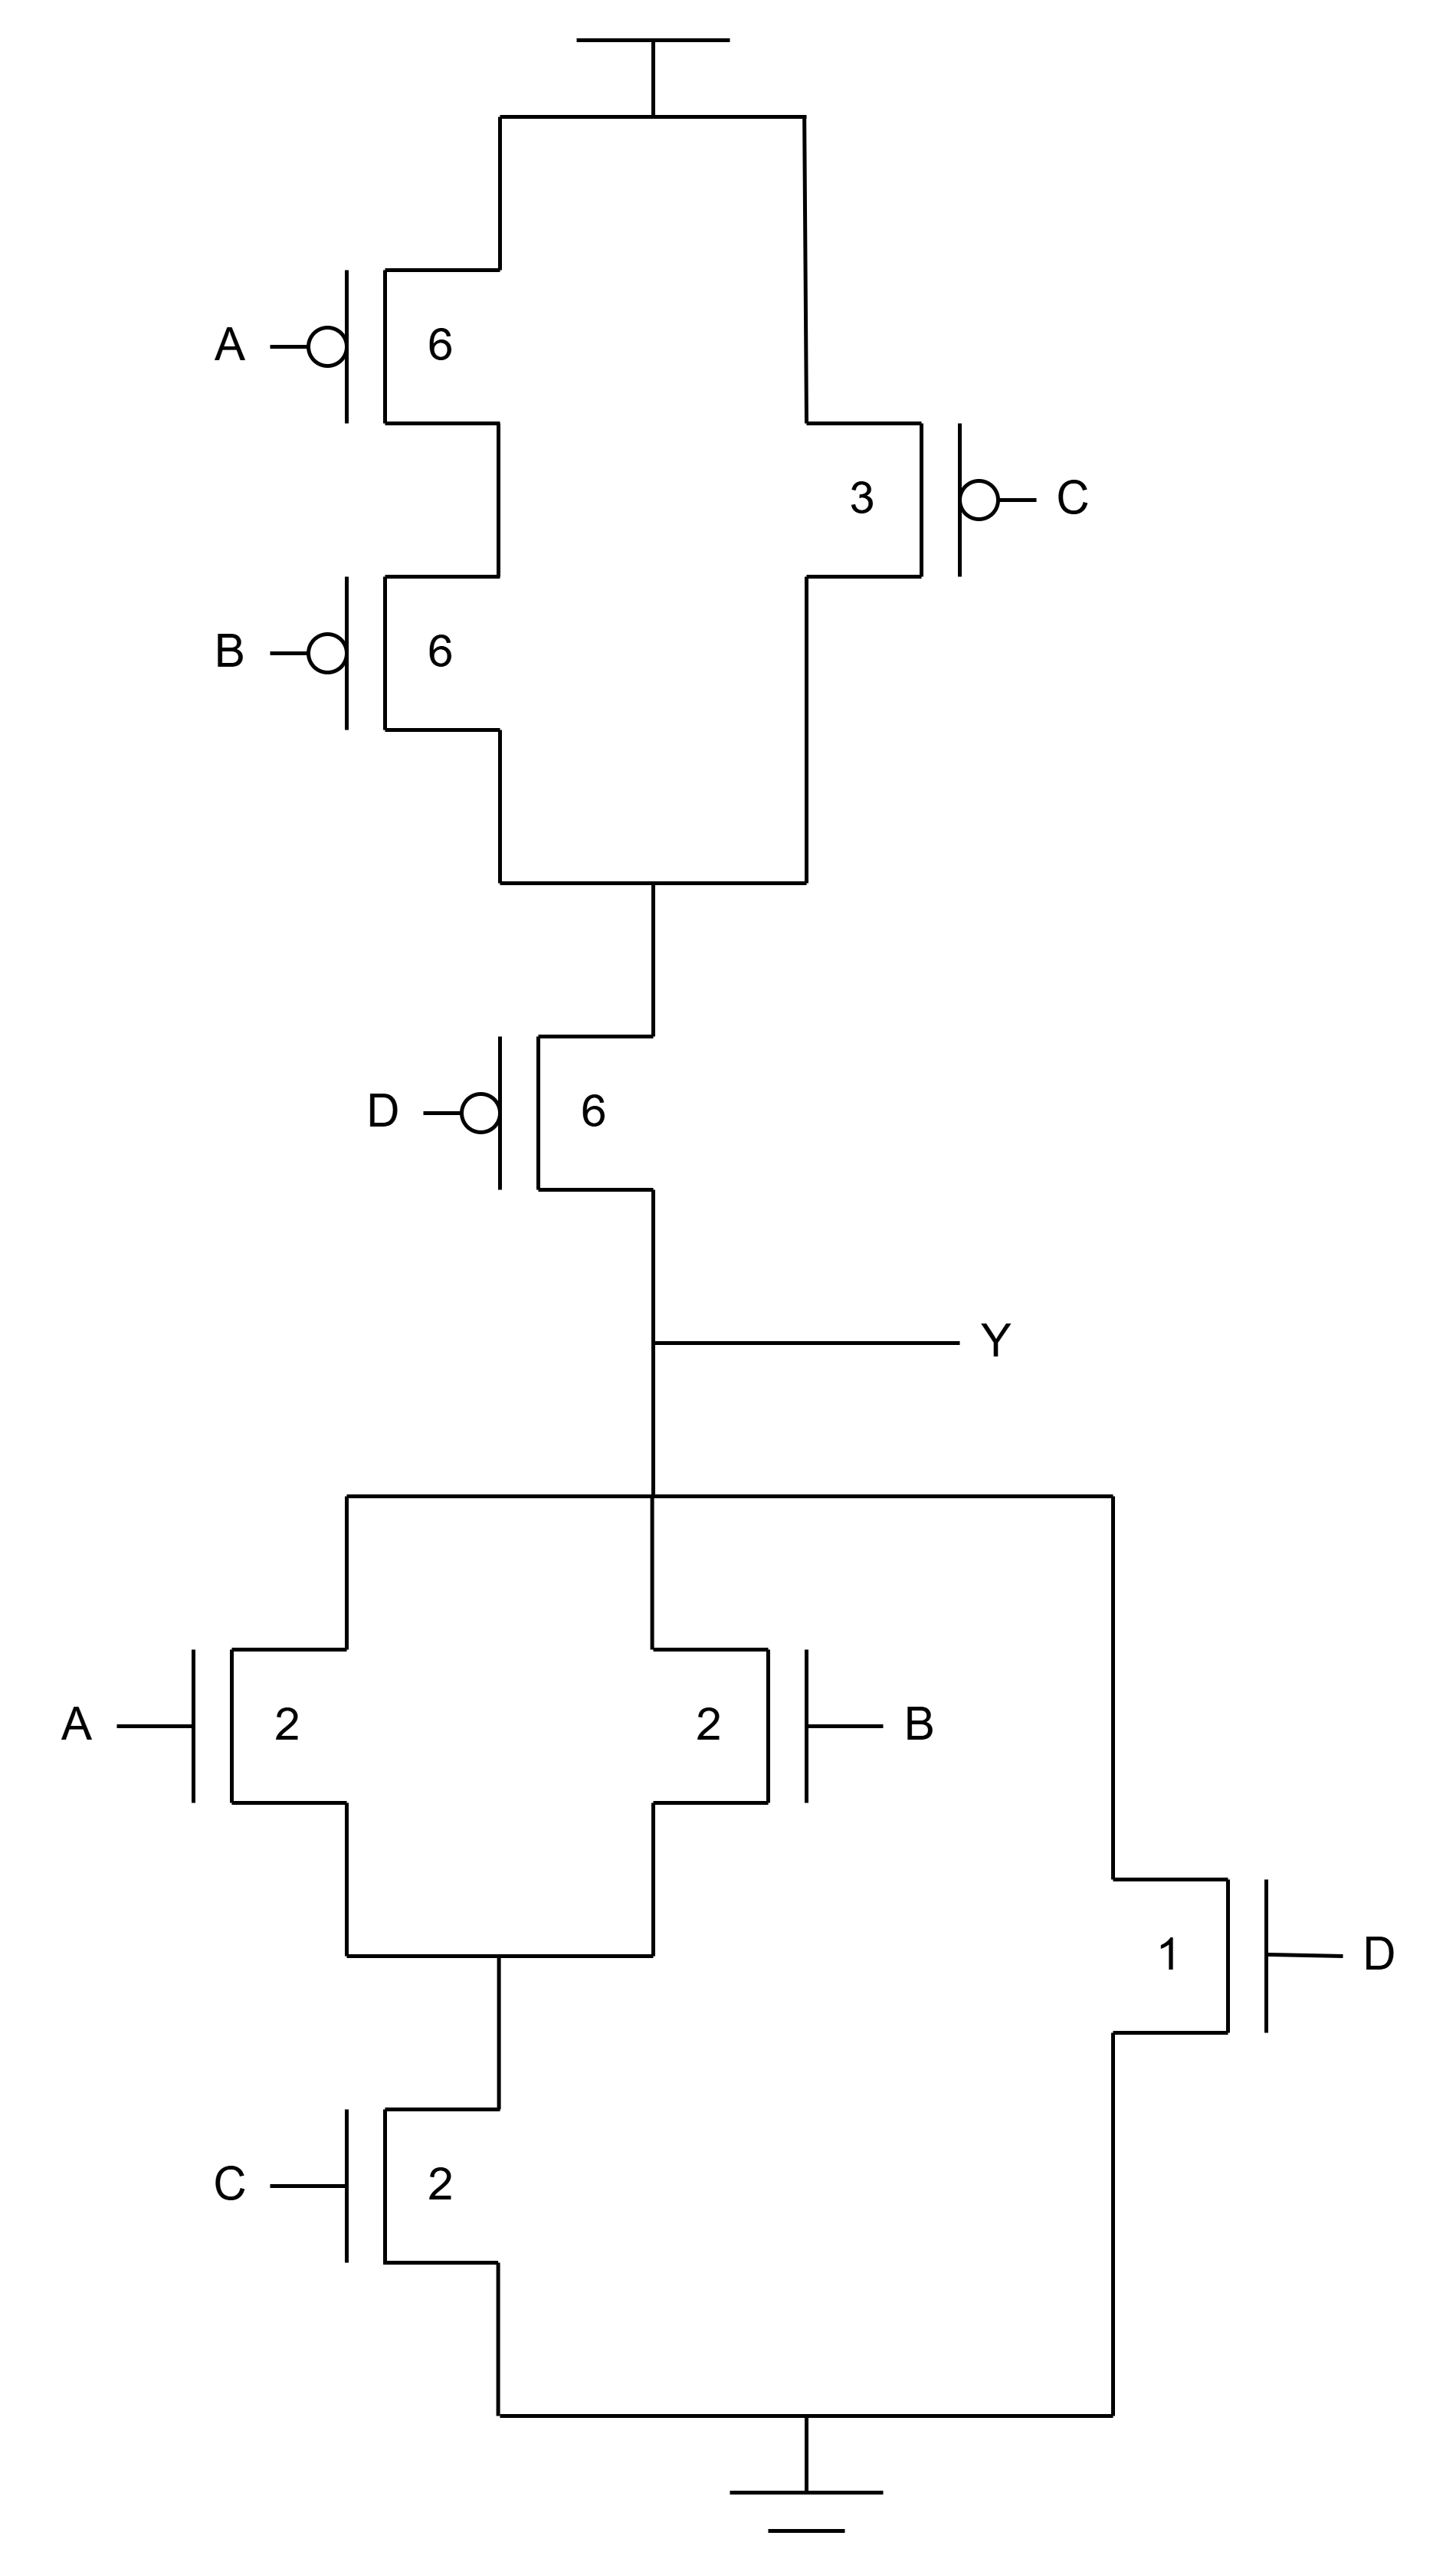
\includegraphics[width=0.35\textwidth]{problem2_static_cmos.png}}
			\caption{Static Complementary CMOS Design which Implements $Y = \overline{(A + B)C + D}$}
			\label{fig::problem2_static_cmos}
		\end{figure}

		Next, we show the pseudo-NMOS design in Figure \ref{fig::problem2_pseudo_nmos}. To get the pseudo NMOS design, we replace the pull-up network, with a single pull-up transistor that is always on. The effective size of the pull-up transistor is decreased, so it can be overcome by the pull-down network when the pull-down network is on.
		
		\begin{figure}[H]
			\centerline{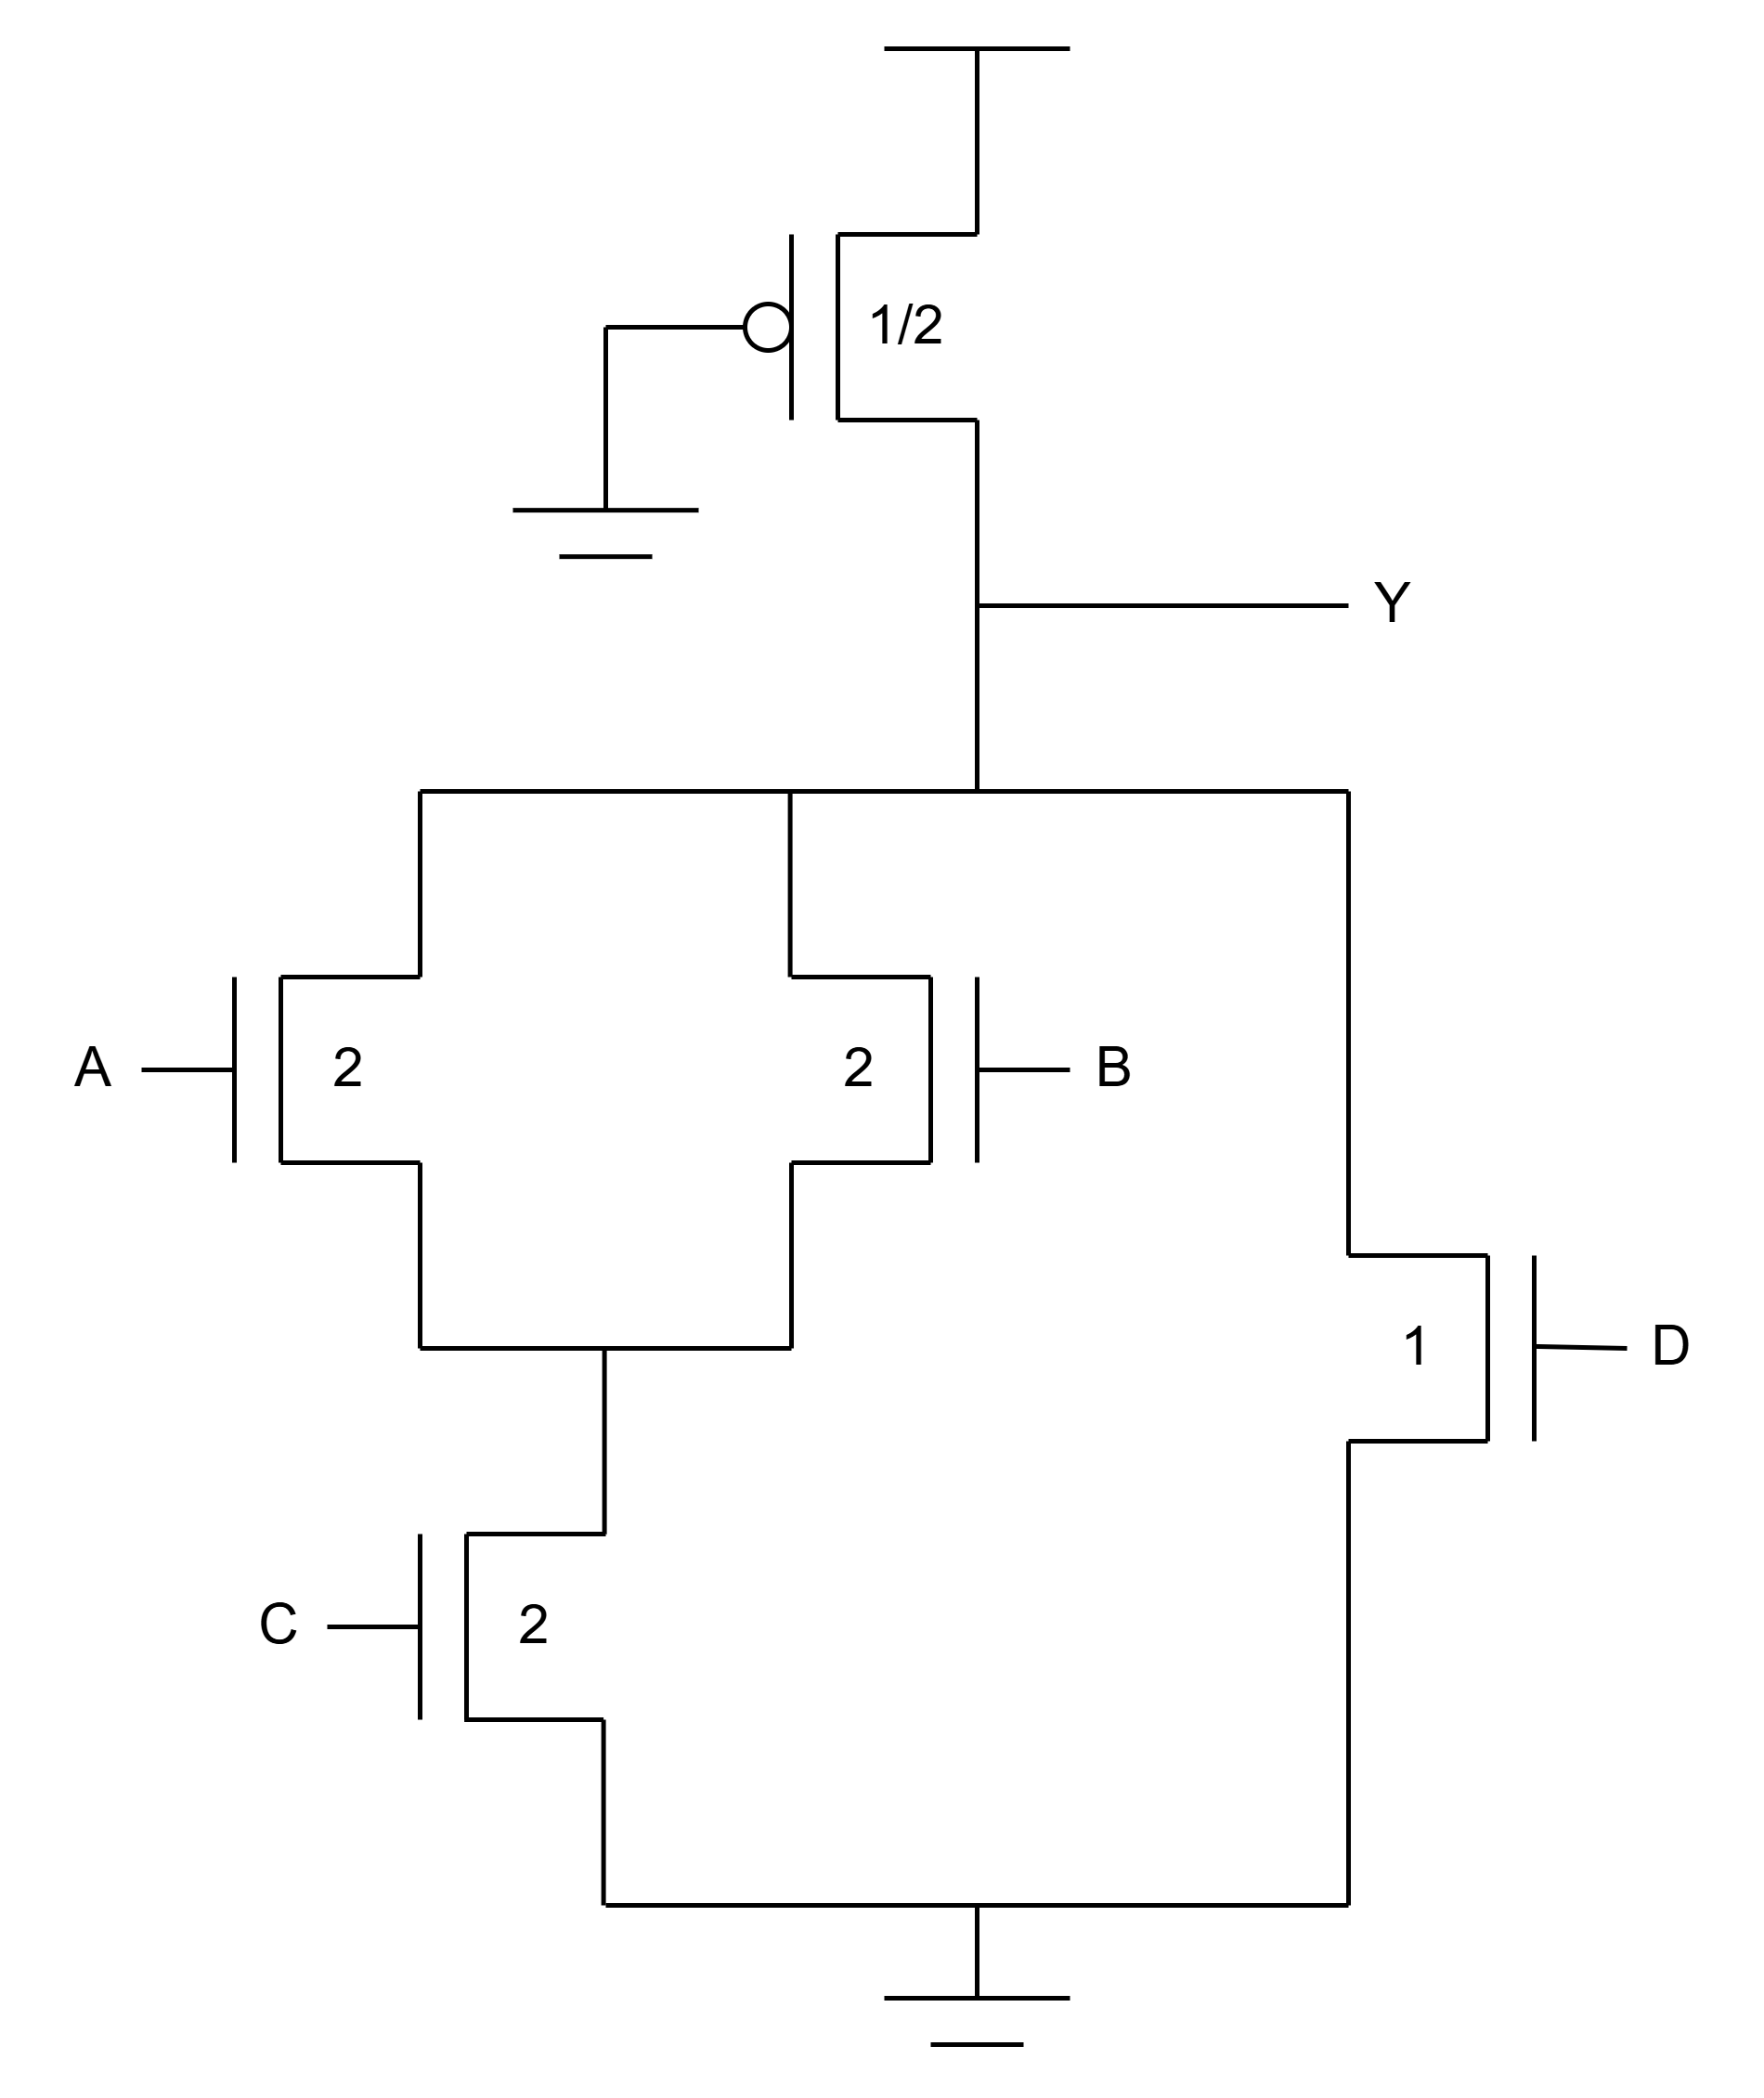
\includegraphics[width=0.35\textwidth]{problem2_pseudo_nmos.png}}
			\caption{Pseudo NMOS Design which Implements $Y = \overline{(A + B)C + D}$}
			\label{fig::problem2_pseudo_nmos}
		\end{figure}

		The pseudo-NMOS circuit has a smaller area and load than the static complementary CMOS design. However, there is more static power dissipation. We can reduce the static power consumption with a domino dynamic circuit. The domino dynamic design is shown in Figure \ref{fig::problem2_domino_dynamic}. In the domino dynamic design, we connect the PMOS transistor to the clock instead of ground. We also add a foot (NMOS transistor connected to the clock) to reduce static power consumption. When the clock is low, we charge the load transistor. Then, when the clock goes high, we evaluate the pull-down network.
		
		\begin{figure}[H]
			\centerline{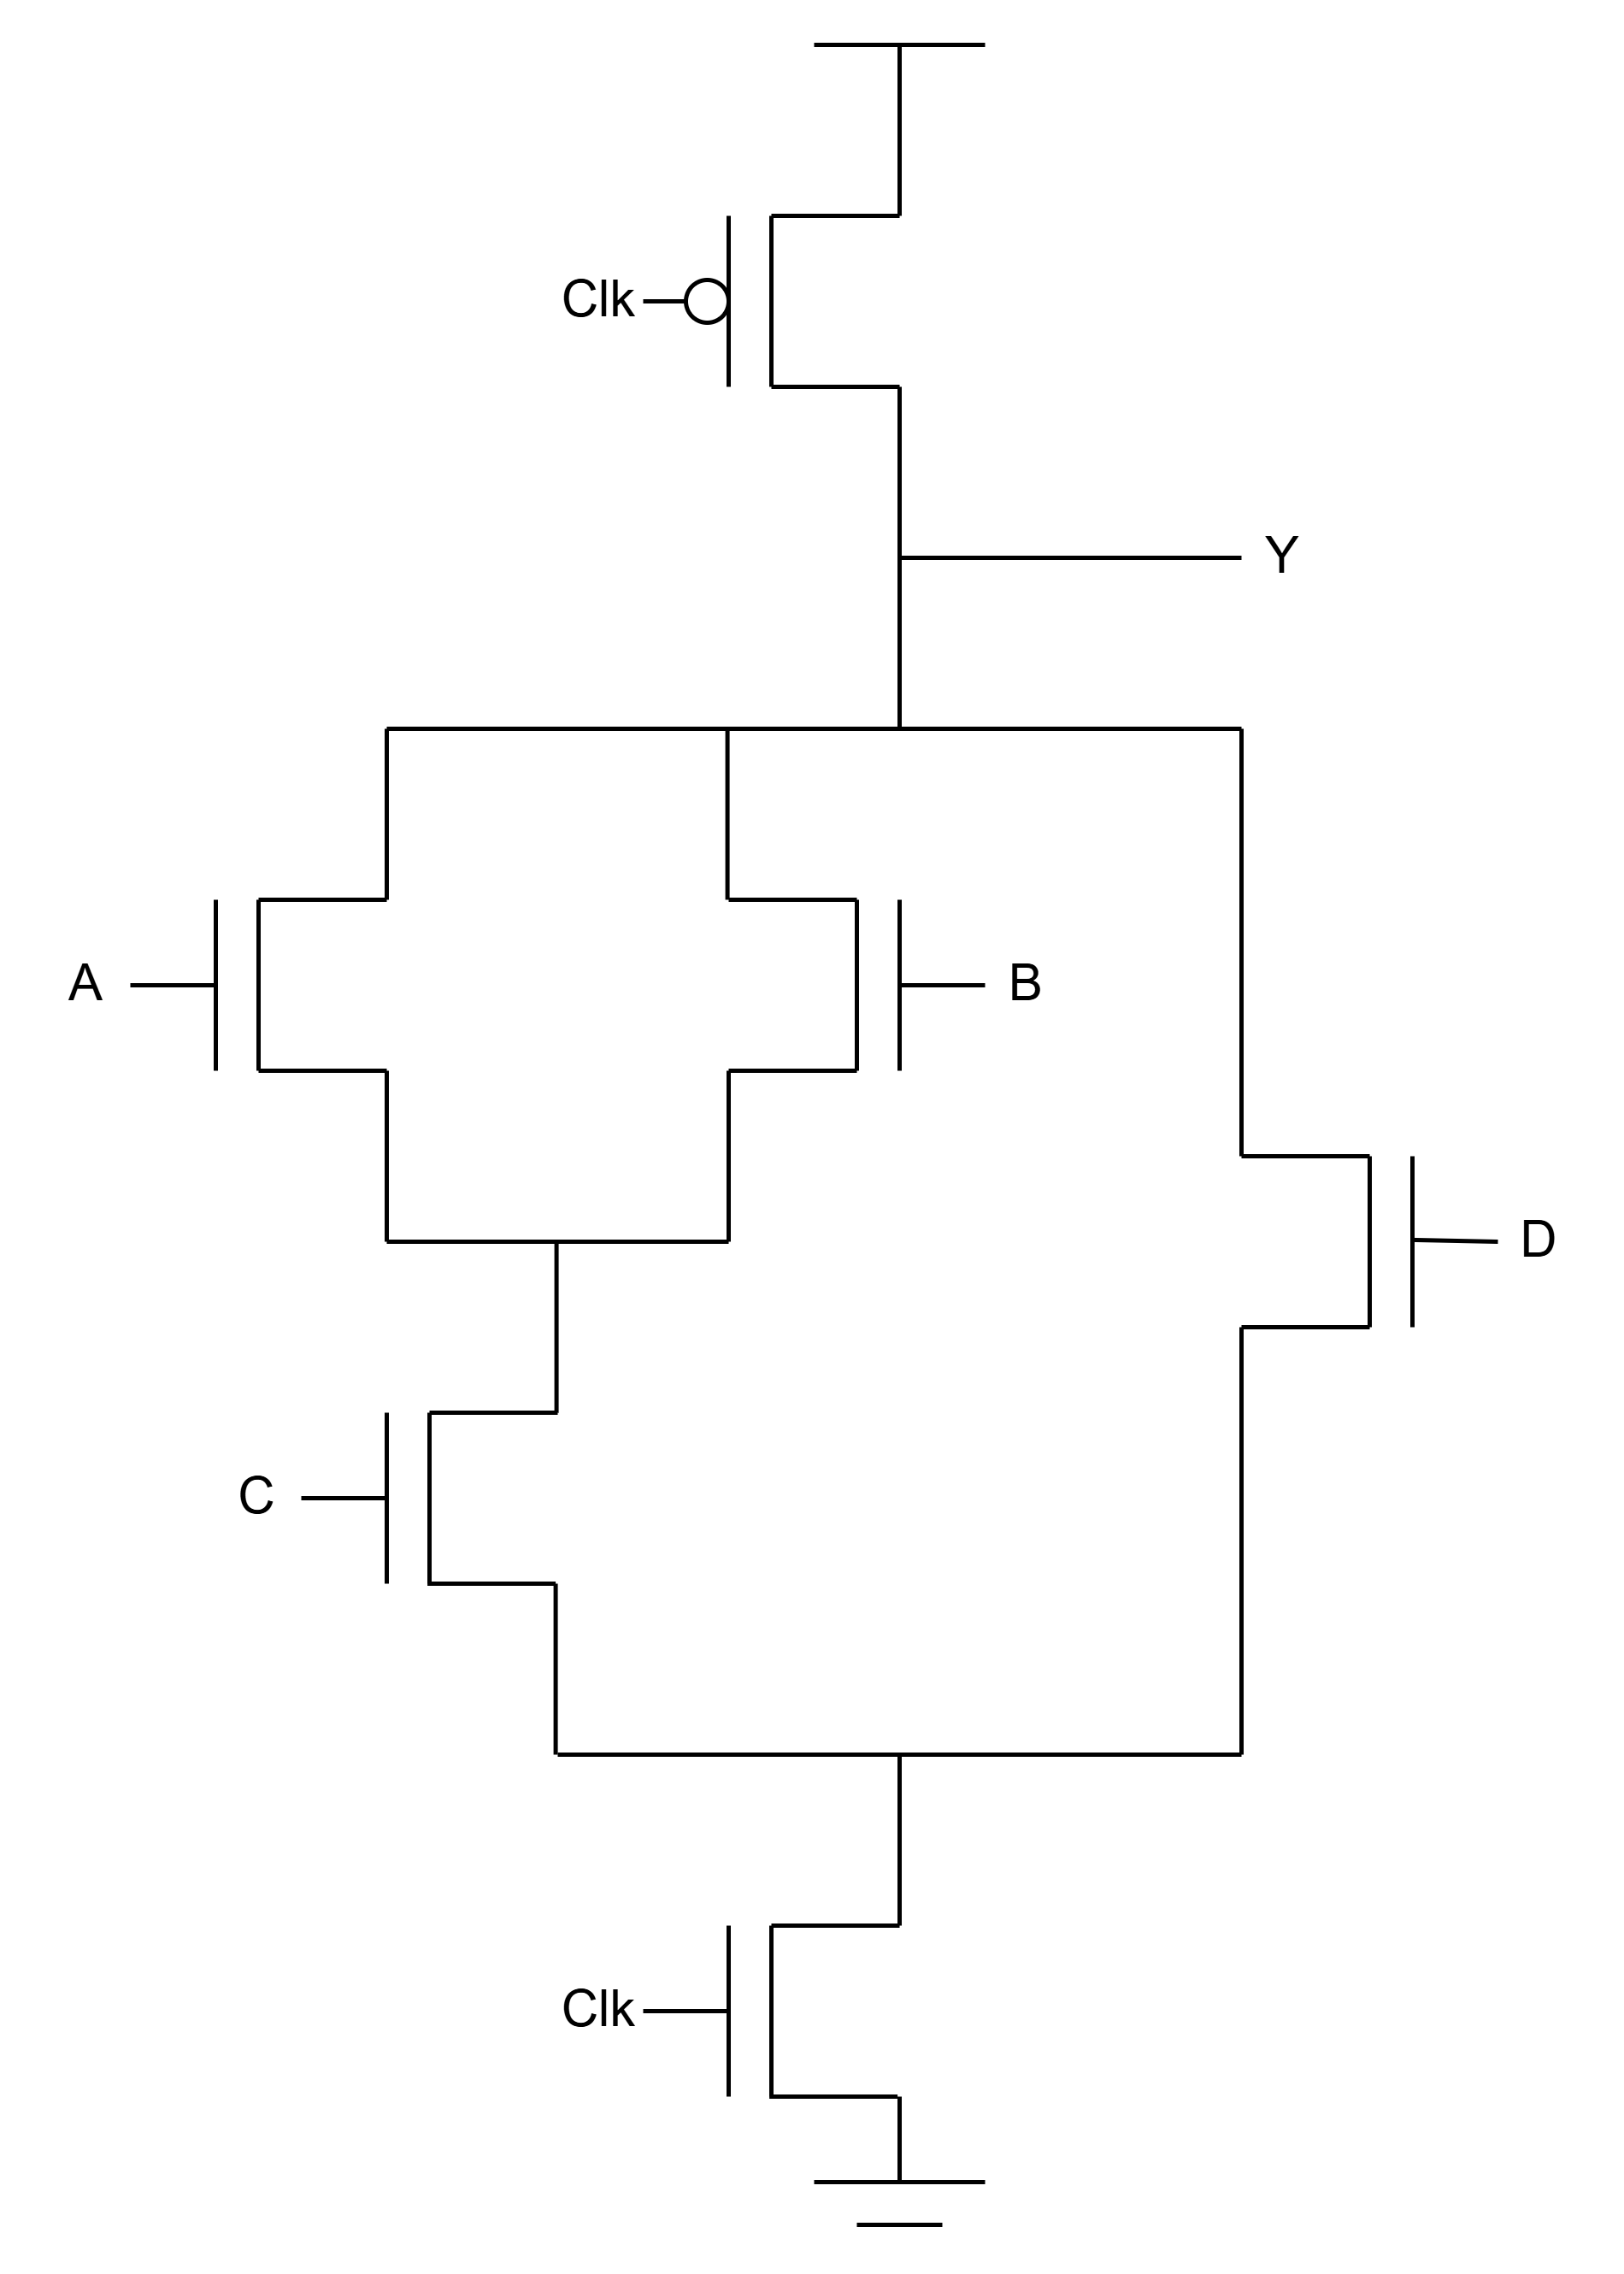
\includegraphics[width=0.35\textwidth]{problem2_domino_dynamic.png}}
			\caption{Domino Dynamic Design which Implements $Y = \overline{(A + B)C + D}$}
			\label{fig::problem2_domino_dynamic}
		\end{figure}

		Domino logic is attractive for high-speed circuits because it reduces the input capacitance (it is 1.3 - 2x faster than static CMOS). However, it has many challenges, which include monotonicity, leakage, charge sharing, and noise. Because power is the limiting factor, it has been widely displaced by static CMOS.
		
		\item In the following figure, what king of logic is implemented in this circuit? Write out the Z function.
		
			\begin{figure}[H]
				\centerline{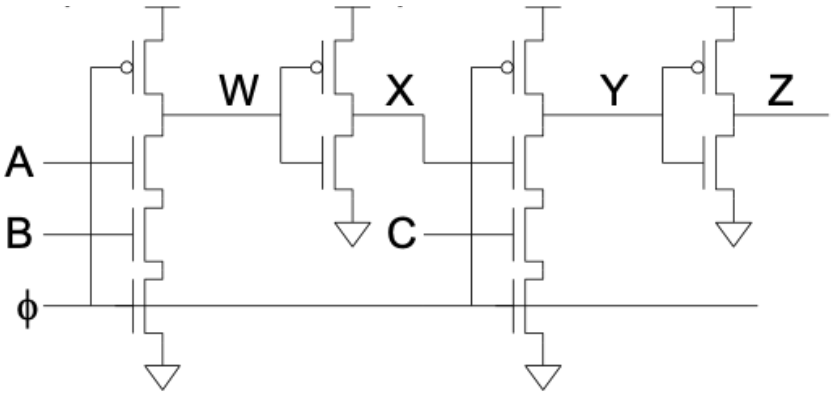
\includegraphics[width=0.5\textwidth]{circuit_question3.png}}
				\label{fig::circuit_question3}
			\end{figure}

			The circuit implements domino dynamic logic.
			
			The dynamic logic gates implement the following equations:
			
			$W = \overline{AB}$
			
			$Y = \overline{XC}$
			
			The static CMOS gates implement the following equations:
			
			$X = \overline{W}$
			
			$Z = \overline{Y}$
			
			$\therefore$ Z can be computed as follows:
			
			$Z = \overline{\overline{XC}} = XC = \overline{W}C = \overline{\overline{AB}}C = \mathbf{ABC}$
			
			Alternatively, we can recognize Z as two chained domino AND gates, which implies
			
			$\mathbf{Z = (AB)C = ABC}$.
			
		\item ~
		
			\begin{enumerate}
			
			\item[1.] What is the size of each transistor for $Y = \overline{AB + C}$ if we use static complementary design?
			
			In the static complementary design, we size the transistors to get the same drive as a unit inverter. For series connections, this means that the width of the transistors need to be doubled to get the same equivalent resistance. For the parallel connections, we consider only the case when one branch is on and don't increase the width of the transistor. In Figure \ref{fig::circuit4a}, we show the static complementary design and the sizes of each transistors.
			
			\begin{figure}[H]
				\centerline{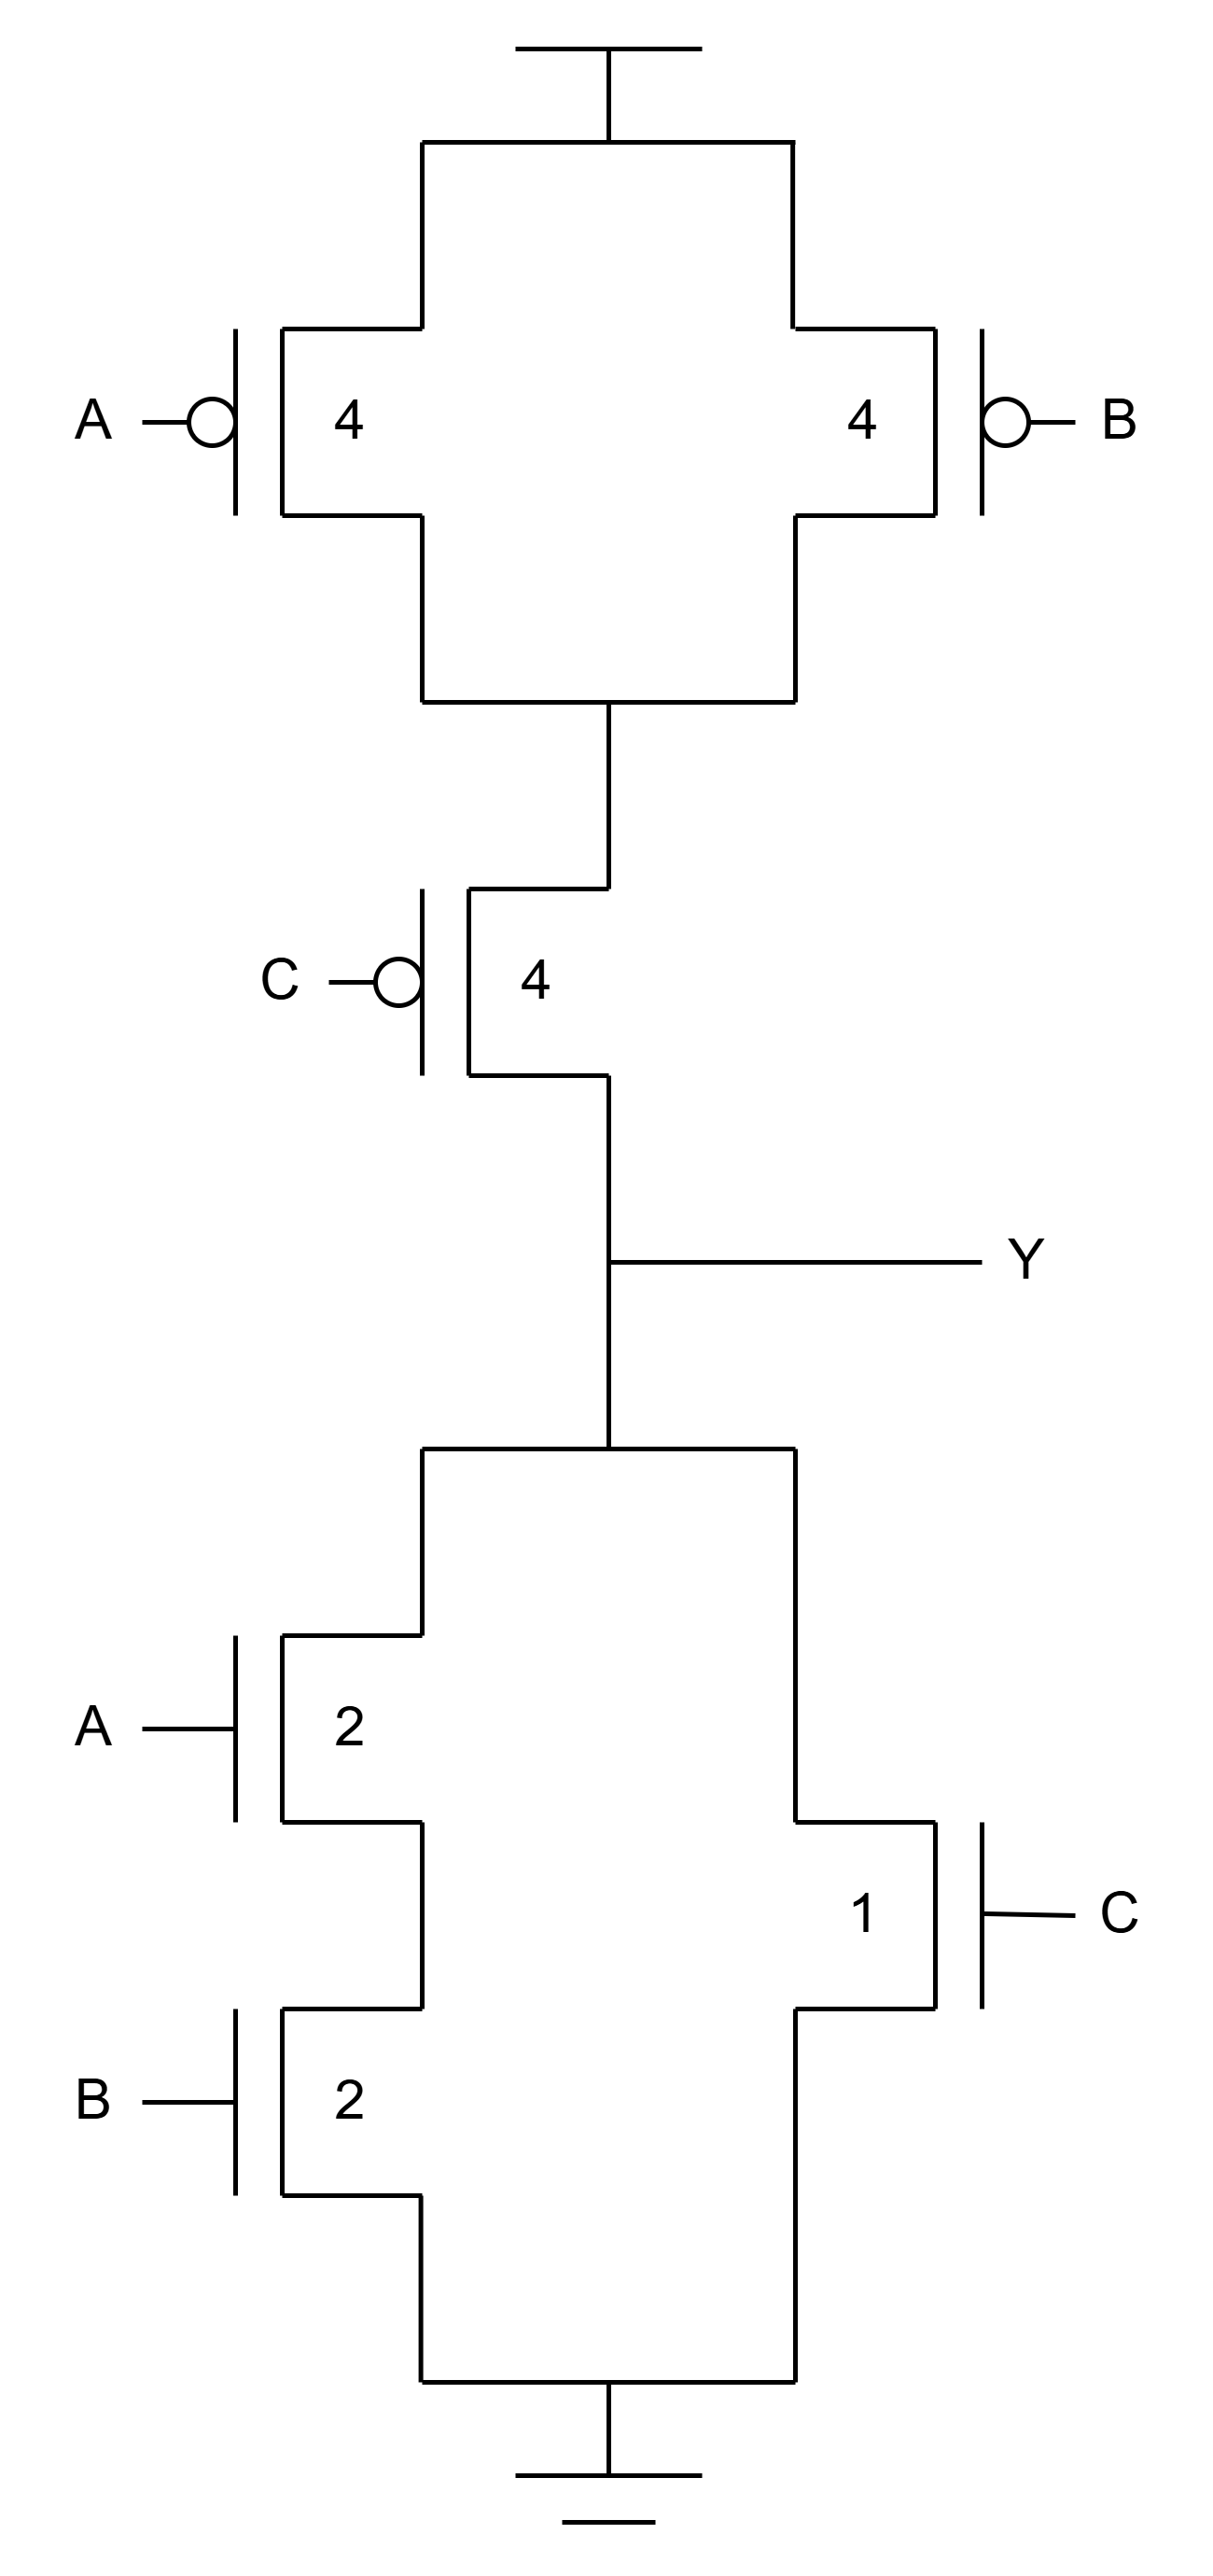
\includegraphics[width=0.25\textwidth]{circuit4a.png}}
				\caption{Static Complementary Design for $Y = \overline{AB + C}$.}
				\label{fig::circuit4a}
			\end{figure}
			
			\item[2.] What type of CMOS design is the depicted in the figure below? Describe its functionality and write down its logic equation?
			
			\begin{figure}[H]
				\centerline{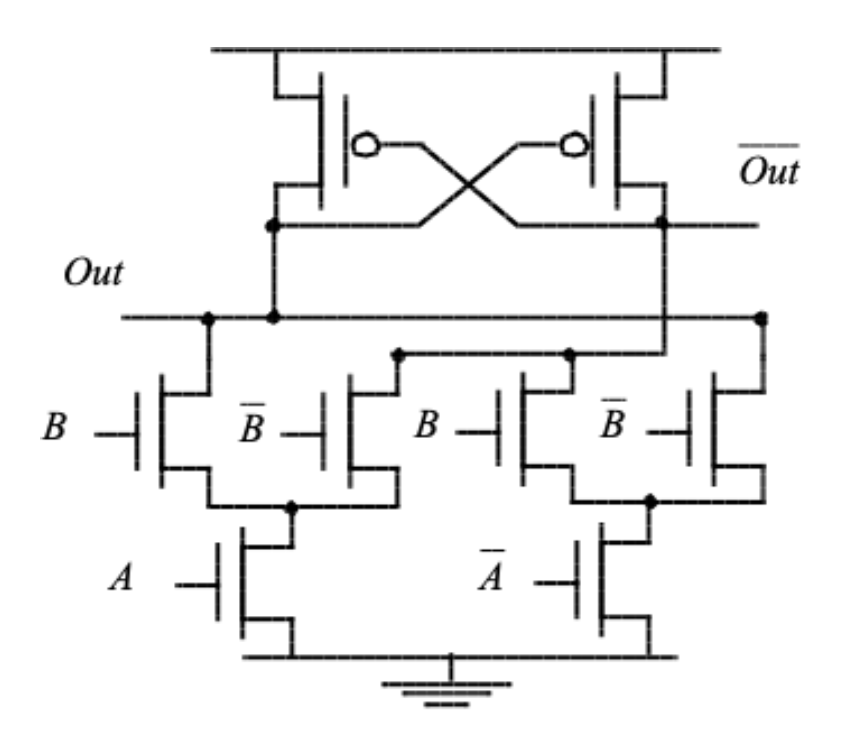
\includegraphics[width=0.5\textwidth]{circuit4b.png}}
				\label{fig::circuit4b}
			\end{figure}
			
			The design illustrates differential cascode voltage switch logic (DCVSL). When A=1 and B=0, $\overline{\text{Out}}$ is connected to ground, and the PMOS transistor on the left is turned on pulling $\text{Out}$ to $V_{DD}$. Similarly, when A=0 and B=1, $\overline{\text{Out}}$ is connected to ground, and the PMOS transistor on the left is turned on pulling $\text{Out}$ to $V_{DD}$. Next, if A=B=0, $\text{Out}$ is connected to ground and the PMOS transistor on the right is turned on pulling $\overline{\text{Out}}$ to $V_{DD}$. Finally, if A=B=1, $\text{Out}$ is connected to ground and the PMOS transistor on the right is turned on pulling $\overline{\text{Out}}$ to $V_{DD}$. Our circuit implements the following logic equations:
			
			\begin{equation*}
				\text{Out} = \bar{A}B + A\bar{B}
			\end{equation*}
			
			\begin{equation*}
				\overline{\text{Out}} = AB + \bar{A}\bar{B}
			\end{equation*}
			
			We recognize the equation for $\text{Out}$ as XOR, and the equation for $\overline{\text{Out}}$ as XNOR. Therefore, our gate implements XOR/XNOR.
			
			\end{enumerate}
			
		\item Setup and Hold time for A?
		
			\begin{figure}[H]
				\centerline{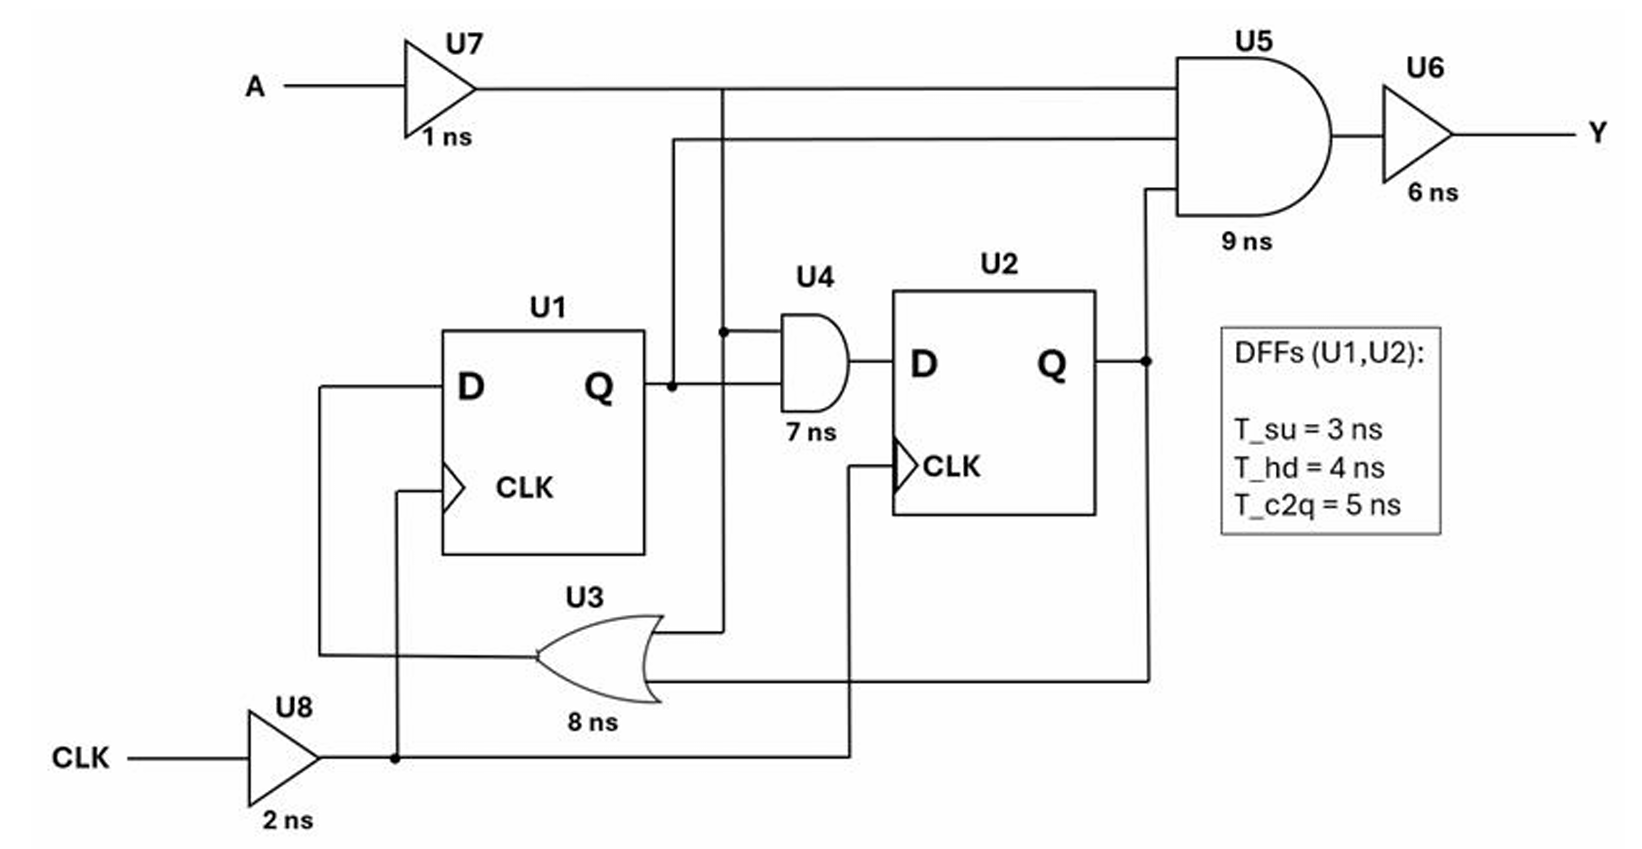
\includegraphics[width=0.5\textwidth]{circuit5.png}}
				\label{fig::circuit5}
			\end{figure}
			
			The setup time for A is the minimum amount of time A must be stable before the rising edge of the clock cycle to ensure the previous input is not accidentally sampled.
			
			$t_{\text{setup}}(A) = \text{Setup Time of Flip Flop} + \text{Max Data path delay} - \text{Min Clock path delay}$
			
			$ = t_{\text{setup}}(U1) + t_{\text{max}}(U7) + t_{\text{max}}(U3) - t_{\text{min}}(U8) = 1\text{ns} + 8\text{ns} + 3\text{ns} - 2\text{ns} = \mathbf{10\text{\textbf{ns}}}$
			
			The hold time for A is the minimum amount of time A must be held after the rising edge of the clock cycle to ensure the next input is not accidentally sampled.
			
			$t_{\text{hold}}(A) = \text{Hold Time of Flip Flop} + \text{Max Clock path delay} - \text{Min Data path delay}$
			
			$ = t_\text{hold}(U2) + t_{\text{max}}(U8) - t_{\text{min}}(U7) - t_{\text{min}}(U4) = 4\text{ns} + 2\text{ns} - 1\text{ns} - 7\text{ns} = \mathbf{-2\text{\textbf{ns}}}$
	\end{enumerate}

\end{document}